\documentclass[fleqn]{article}
\oddsidemargin 0.0in
\textwidth 6.0in
\thispagestyle{empty}
\usepackage{import}
\usepackage{amsmath}
\usepackage{graphicx}
\usepackage{flexisym}
\usepackage{amssymb}
\usepackage{bigints} 
\usepackage[english]{babel}
\usepackage[utf8x]{inputenc}
\usepackage{float}
\usepackage[colorinlistoftodos]{todonotes}

\definecolor{hwColor}{HTML}{042c4d}
\setlength\parindent{24pt}

\begin{document}

  \begin{titlepage}

    \newcommand{\HRule}{\rule{\linewidth}{0.5mm}}

    \center


    \textsc{\LARGE Arizona State University}\\[1.5cm]

    \textsc{\LARGE Advanced Calculus I }\\[1.5cm]


    \begin{figure}
      
\includegraphics[width=\linewidth]{asu.png}
    \end{figure}


    \HRule \\[0.4cm]
    { \huge \bfseries Homework Four }\\[0.4cm] 
    \HRule \\[1.5cm]

    \textbf{Behnam Amiri}

    \bigbreak

    \textbf{Prof: Sergei Suslov}

    \bigbreak


    \textbf{{\large \today}\\[2cm]}

    \vfill

  \end{titlepage}

  \textbf{4.1 THE DERIVATIVE OF A FUNCTION }
  \begin{enumerate}
    \item (2) Prove that the definition of the derivative and the alternate definition of the derivative are
    equivalent.

      \textcolor{hwColor}{
        \hspace{15pt} Let's start off by remembering what the definition of the derivative and the alternate definition are.
        \\
        \\
        \textbf{The definition of the derivative:}
        \\
        The function $f$ is said to be differentiable at $x_0$ iff $\dfrac{f(x)-f(x_0)}{x-x_0}$ has a limit at $x_0$
        and we write $$f^'(x_0)=\lim\limits_{x \to x_0} \dfrac{f(x)-f(x_0)}{x-x_0}$$
        \\
        \textbf{The alternate definition of the derivative:}
        \\
        The function $f$ is said to be differentiable at $x_0$ iff $\dfrac{f(x_0+t)-f(x_0)}{t}$ has a limit at 
        zero. If this limit exists, it is called the derivative of $f$ at $x_0$.
        \\
        \\
        Even though the two definitions seem different but if we look carefully they are the same indeed.
        \\
        \\
        \emph{\textbf{Proof:}}
        \\
        \\
        Suppose $x=x_0+t$ then we can have the following:
        \\
        \\
        $
          \lim\limits_{t \to 0} \dfrac{f(x_0+t)-f(x_0)}{t}
          \\
          \\
          =\lim\limits_{x-x_0 \to 0} \dfrac{f(x)-f(x_0)}{x-x_0}
          \\
          \\
          =\lim\limits_{x \to x_0} \dfrac{f(x)-f(x_0)}{x-x_0}
          \\
          \\
          \\
          \therefore ~~~~ \lim\limits_{t \to 0} \dfrac{f(x_0+t)-f(x_0)}{t}=\lim\limits_{x \to x_0} \dfrac{f(x)-f(x_0)}{x-x_0} ~~~~~~~~~ \blacksquare
          \\
        $
      }

    \item (3) Use the definition to find the derivative of $f(x)=\sqrt{x}$, for $x > 0$. Is $f$ differentiable at zero? Explain.

      \textcolor{hwColor}{
        \\
        The definiton is defined as $f^'(x_0)=\lim\limits_{x \to x_0} \dfrac{f(x)-f(x_0)}{x-x_0}$ we have:
        \\
        \\
        $
          f^'(x_0)=\lim\limits_{x \to 0} \dfrac{f(x)-f(0)}{x-0}
          \\
          \\
          =\lim\limits_{x \to x_0} \dfrac{\sqrt{x}-\sqrt{0}}{x-0}
          \\
          \\
          =\lim\limits_{x \to x_0} \dfrac{\sqrt{x}}{x}
          \\
          \\
        $
        With the help of L’H\^{o}pital’s Rule we have:
        \\
        \\
        $
          =\lim\limits_{x \to x_0} \dfrac{\dfrac{1}{2\sqrt{x}}}{1}
          \\
          \\
          =\dfrac{1}{2\sqrt{x_0}}
          \\
          \\
          \\
          \therefore ~~~~ f^'(0)=+\infty ~~~~ \checkmark 
        $
        \\
        \\
        It is not differentiable, because the derivative of $f$ at zero tends to $+\infty$ as it was shown. 
        By using the alternate definition of the derivative we have:
        \\
        \\
        $
          f^'(x_0)=\lim\limits_{t \to 0} \dfrac{f(x_0+t)-f(x_0)}{t}
          \\
          \\
          =\lim\limits_{t \to 0} \dfrac{\sqrt{x_0+t}-\sqrt{x_0}}{t}
          \\
          \\
          =\lim\limits_{t \to 0} \dfrac{\sqrt{x_0+t}-\sqrt{x_0}}{t} \times \dfrac{\sqrt{x_0+t}+\sqrt{x_0}}{\sqrt{x_0+t}+\sqrt{x_0}}
          \\
          \\
          =\lim\limits_{t \to 0} \dfrac{x_0+t-x_0}{t \left(\sqrt{x_0+t}+\sqrt{x_0}\right)}
          \\
          \\
          =\lim\limits_{t \to 0} \dfrac{t}{t\left(\sqrt{x_0+t}+\sqrt{x_0}\right)}
          \\
          \\
          =\lim\limits_{t \to 0} \dfrac{1}{\sqrt{x_0+t}+\sqrt{x_0}}
          \\
          \\
          =\dfrac{1}{2\sqrt{x_0}}
          \\
          \\
          \\
          \therefore ~~~~ f^'(0)=+\infty ~~~~ \checkmark 
        $
        \\
        \\
        As we expected we got the same result which is function $f$ is not differentiable at zero. $~~~~ \checkmark$
        \\
      }

    \item (4) Use the definition to find the derivative of $g(x)=x^2$.

      \textcolor{hwColor}{
        We know the definition is $g^'(x_0)=\lim\limits_{t \to 0} \dfrac{f(x_0+t)-f(x_0)}{t}$ and $g(x)=x^2$ so
        we have the following:
        \\
        \\
        $
          g^'(x_0)=\lim\limits_{t \to 0} \dfrac{f(x_0+t)-f(x_0)}{t}
          \\
          \\
          =\lim\limits_{t \to 0} \dfrac{\left(x_0+t\right)^2-x_0^2}{t}
          \\
          \\
          =\lim\limits_{t \to 0} \dfrac{x_0^2+2x_0t+t^2-x_0^2}{t}
          \\
          \\
          =\lim\limits_{t \to 0} \dfrac{t \left(2x_0+t\right)}{t}
          \\
          \\
          =\lim\limits_{t \to 0} 2x_0+t
          \\
          \\
          \\
          \therefore ~~~~ g^'(x_0)=2x_0 ~~~~ \checkmark
        $
      }

    \item (6) Suppose $f: (a, b) \longrightarrow R$ is differentiable at $x \in (a, b)$. Prove that 
    $$
      \lim\limits_{h \to 0} \dfrac{f(x+h)-f(x-h)}{2h}
    $$
    exists and equals $f^'(x)$. Give an example of a function where this limit exists, but the
    function is not differentiable.

      \textcolor{hwColor}{
        According to the textbook, a function $f$ is said to be differentiable at $x_0$ or has
        a derivative at $x_0$ iff $\lim\limits_{t \to 0} \dfrac{f(x_0+t)-f(x_0)}{t}$ exists at $x_0$.
        \\
        \\
        So let's start with the given statement to see where it can take us.
        \\
        \\
        $
          \lim\limits_{h \to 0} \dfrac{f(x+h)-f(x-h)}{2h}
          \\
          \\
          =\lim\limits_{h \to 0} \dfrac{f(x+h)-f(x-h)+f(x)-f(x)}{2h}
          \\
          \\
          =\lim\limits_{h \to 0} \left[\dfrac{f(x+h)-f(x)}{2h}+\dfrac{-f(x-h)+f(x)}{2h}\right]
          \\
          \\
          =\lim\limits_{h \to 0} \left[\dfrac{f(x+h)-f(x)}{2h}+\dfrac{f(x-h)-f(x)}{-2h}\right]
          \\
          \\
          =\dfrac{1}{2} \left[\lim\limits_{h \to 0}\dfrac{f(x+h)-f(x)}{h}+\lim\limits_{h \to 0}\dfrac{f(x-h)-f(x)}{-h}\right]
          \\
          \\
          =\dfrac{1}{2} \left[f^'(x)+f^'(x)\right]
          \\
          \\
          \\
          \therefore ~~~~ \lim\limits_{h \to 0} \dfrac{f(x+h)-f(x-h)}{2h} \Longleftrightarrow f^'(x) ~~~~ \checkmark
        $
        \\
        \\
        \\
        An example of a function that is continuous but non differentiable at zero is $f(x)=|x|$.
        \\
        \\
        $
          \lim\limits_{h \to 0} \dfrac{f(0+h)-f(0-h)}{2h}
          \\
          \\
          =\lim\limits_{h \to 0} \dfrac{|0+h|-|0-h|}{2h}
          \\
          \\
          \\
          \therefore ~~~~ \lim\limits_{h \to 0} \dfrac{f(0+h)-f(0-h)}{2h}=0
        $
        \\
        \\
        Based off of the result, the limit of $f$ at $x=0$ is zero. (its limit exists) but $f$ is not differentiable at zero.
        \\
        \\
        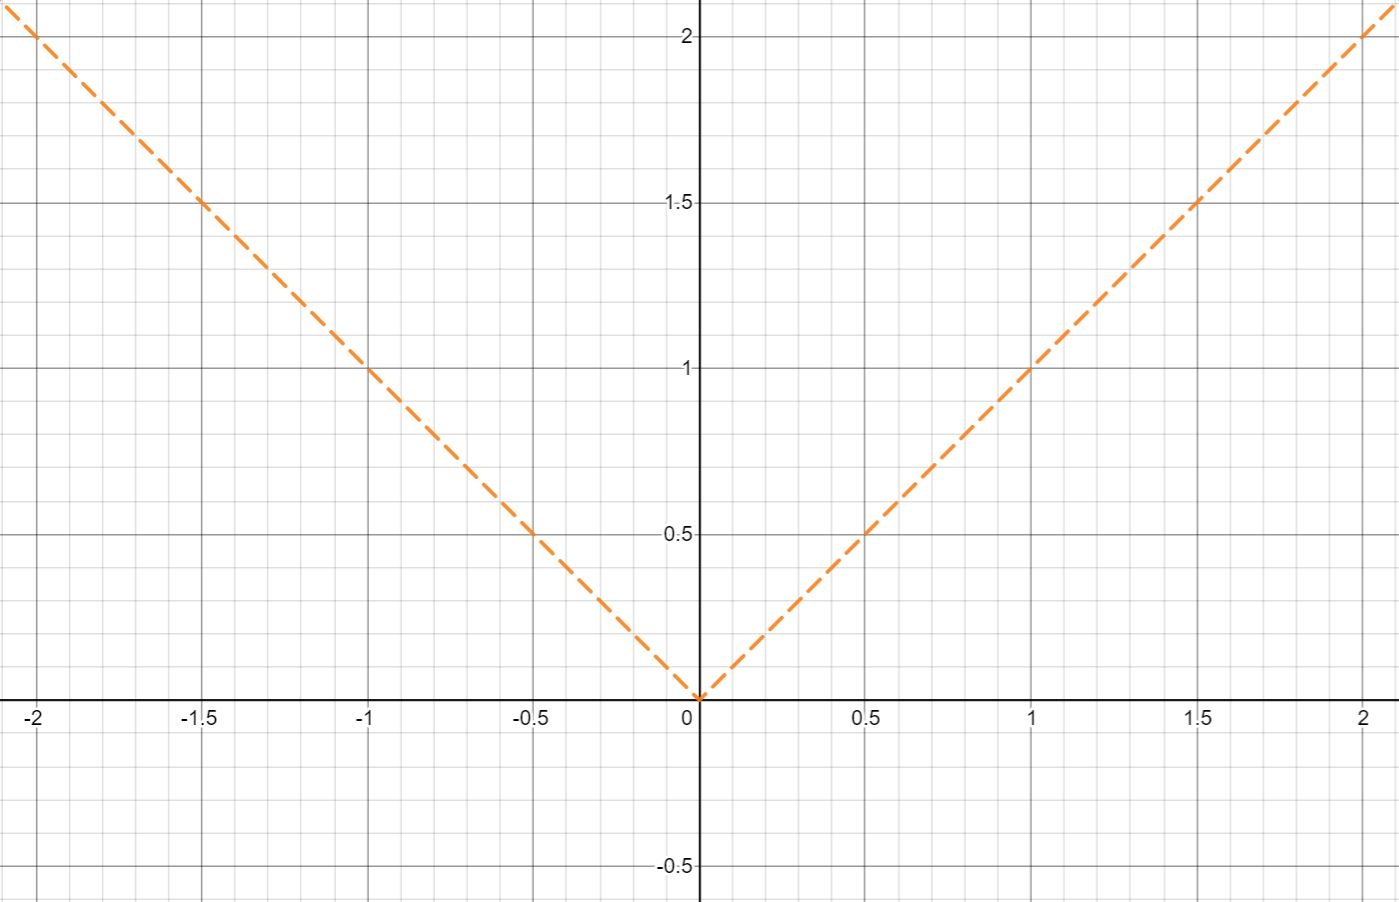
\includegraphics[height=5cm, width=9cm]{absoluteValueFunction.JPG}
      }


  \end{enumerate}

  \rule{15cm}{1pt}

  \textbf{4.2  THE ALGEBRA OF DERIVATIVES}
  \begin{enumerate}
    \item (11) Prove $f: (0, 1) \longrightarrow R$ defined by $f(x)=\sqrt{2x^2-3x+6}$ is differentiable on $(0, 1)$ and 
    compute the derivative.

      \textcolor{hwColor}{
        On page $119$ of the textbook, we learned that \emph{If $f$ is differentiable at $x_0$ and $g$ is differentiable at $f(x_0)$, then $gof$ is differentiable at $x_0$}.
        (Chain rule)
        $$
          \left(gof\right)^'(x_0)=g^'\left(f(x_0)\right) f^'(x_0)
        $$
        Let's assume $g(x)=2x^2-3x+6$ and $w(x)=\sqrt{x}$. We know that both $g(x)$ and $w(x)$ are differentiable, so does 
        their composition $\left(gow\right)$ therefore:
        \\
        \\
        $
          f^'(x)=\dfrac{d}{dx}(gow)
          \\
          \\
          =\dfrac{d}{dx} g\left(w(x)\right)
          \\
          \\
          =\dfrac{d}{dx} \left(2x^2-3x+6\right) \times \dfrac{d}{dx} \left(\sqrt{2x^2-3x+6}\right)
          \\
          \\
          =\left(4x-3\right) \times \dfrac{1}{2\sqrt{2x^2-3x+6}}
          \\
          \\
          \\
          \therefore ~~~~ f^'(x)=\dfrac{4x-3}{2\sqrt{2x^2-3x+6}} ~~~~ \checkmark
        $
      }

    \item (14) Suppose $f: R \longrightarrow R$ is differentiable and define $g(x)=x^2 f(x^3)$. Show that $g$ is
    differentiable and compute $g^'$.

      \textcolor{hwColor}{
        On page $119$ of the textbook, we learned that \emph{If $f$ is differentiable at $x_0$ and $g$ is differentiable at $f(x_0)$, then $gof$ is differentiable at $x_0$}.
        (Chain rule)
        $$
          \left(gof\right)^'(x_0)=g^'\left(f(x_0)\right) f^'(x_0)
        $$
        The composition of two differentiable functions is also differentiable. We know $x^3$ is differentiable and by the chain rule $f(x^3)$ is differentiable too.
        \\
        \\
        $
          \left(f(x^3)\right)^'
          =\dfrac{d}{dx}x^3 \times f^'(x^3)
          =3x^2 f^'(x^3)
        $
        \\
        \\
        Now we are ready to find $g^'(x)$.
        \\
        \\
        $
          g^'(x)=\dfrac{d}{dx}(x^2) f(x^3)+x^2\dfrac{d}{dx} \left(f(x^3)\right)^
          =2x f(x^3)+x^2 \left[3x^2 f^'(x^3)\right]
          \\
          \\
          \\
          \therefore ~~~~ g^'(x)=2x f(x^3)+3x^4 f^'(x^3) ~~~~ \checkmark
          \\
        $
      }
    
    \item (15) Define $f(x)=\sqrt{x+\sqrt{x+\sqrt{x}}}$ for $x \geq 0$. Determine where $f$ is differentiable and compute
    the derivative. 

      \textcolor{hwColor}{
        \emph{We know that $\sqrt{x}$ is differentiable.}
        \\
        \\
        We can find the derivative of the given function by the chain and addition rules.
        \\
        \\
        $
          \dfrac{df}{dx}=\dfrac{d}{dx} \left[\sqrt{x+\sqrt{x+\sqrt{x}}}\right]
          \\
          \\
          =\dfrac{d}{dx} \left[\left(x+\sqrt{x+\sqrt{x}}\right)^{\dfrac{1}{2}}\right]
          \\
          \\
          =\dfrac{1}{2} \times \dfrac{d}{dx} \left(x+\sqrt{x+\sqrt{x}}\right) \times \left(x+\sqrt{x+\sqrt{x}}\right)^{-\dfrac{1}{2}} ~~~~~ (A)
          \\
          \\
        $
        Now let's find the derivative of $\dfrac{d}{dx} \left(x+\sqrt{x+\sqrt{x}}\right)$ then we can plug it into equation $(A)$.
        \\
        \\
        $
          \dfrac{d}{dx} \left(x+\sqrt{x+\sqrt{x}}\right)
          \\
          \\
          =\dfrac{d}{dx} \left[x+\left(x+\sqrt{x}\right)^{\dfrac{1}{2}}\right]
          \\
          \\
          =1+\dfrac{1}{2} \dfrac{d}{dx} \left[x+\sqrt{x}\right] \left(x+\sqrt{x}\right)^{-\dfrac{1}{2}}
          \\
          \\
          =1+\dfrac{1}{2} \left(1+\dfrac{1}{2\sqrt{x}}\right) \left(x+\sqrt{x}\right)^{-\dfrac{1}{2}}
          \\
          \\
          \\
          \\
          \therefore ~~~~ (A) ~~~~  \dfrac{1}{2} \times \left[1+\dfrac{1}{2} \left(1+\dfrac{1}{2\sqrt{x}}\right) \left(x+\sqrt{x}\right)^{-\dfrac{1}{2}}\right] \times \left(x+\sqrt{x+\sqrt{x}}\right)^{-\dfrac{1}{2}}
          \\
          \\
          \\
          =\dfrac{1}{2 \sqrt{x+\sqrt{x+\sqrt{x}}}}+\dfrac{\left(1+\dfrac{1}{2\sqrt{x}}\right)}{4 \left(x+\sqrt{x+\sqrt{x}}\right)^{\dfrac{1}{2}} \left(x+\sqrt{x}\right)^{\dfrac{1}{2}}}
          \\
          \\
          \\
          \therefore ~~~~ \dfrac{df}{dx}=\dfrac{1}{2 \sqrt{x+\sqrt{x+\sqrt{x}}}}+\dfrac{1+\dfrac{1}{2\sqrt{x}}}{4 \sqrt{x+\sqrt{x+\sqrt{x}}} \sqrt{x+\sqrt{x}}} ~~~~ \checkmark
          \\
        $
      }

  \end{enumerate}

  \rule{15cm}{1pt}

  \textbf{4.3 ROLLE'S THEOREM AND THE MEAN-VALUE THEOREM}
  \begin{enumerate}
    \item (16) Define $f: [0, 2] \longrightarrow R$ by $f(x)=\sqrt{2x-x^2}$. Show that $f$ satisfies the conditions of Rolle's
    theorem and find $c$ such that $f^'(c)=0$.

      \textcolor{hwColor}{
        Rolle's theorem essentially states that any real-valued differentiable 
        function that attains equal values at two distinct points must have at least one stationary 
        point somewhere between them. Recall that in order to be able to apply the Rolle's theorem, three conditions 
        must be met.
        \begin{enumerate}
          \item $[a, b] \longrightarrow$ Continuous.
          \item $(a, b) \longrightarrow$ Differentiable.
          \item $f(a)=f(b)$.
        \end{enumerate}
      }

      \textcolor{hwColor}{
        Suppose $k(x)=2x-x^2$ and $h(x)=\sqrt{x}$. So we can rewrite $f(x)=hok(x)$. We know that both $k(x)$
        and $h(x)$ are differentiable, therefore according to theorem 4.4, $f(x)$ is differentiable as well.
        \\
        \\
        We know that the first two conditions for Rolle's theorem are met. Now let's show the third condition.
        \\
        \\
        $
          \begin{cases}
            f(0)=\sqrt{2(0)-0^2}=0
            \\
            \\
            f(2)=\sqrt{2(2)-2^2}=0
          \end{cases}
          \Longrightarrow f(0)=f(2) ~~~~ \checkmark
        $
        \\
        \\
        Hence, Rolle's theorem is satisfied. Now we know that there must be a number $c$ such that $c \in (a, b)$
        and $f^'(c)=0$.
        \\
        \\
        $
          \dfrac{df}{dx}=\dfrac{d}{dx} \left[\sqrt{2x-x^2}\right]=\dfrac{2-2x}{2 \sqrt{2x-x^2}}=\dfrac{1-x}{\sqrt{2x-x^2}}
          \\
          \\
          \\
          \dfrac{df}{dx}=0 \longrightarrow \dfrac{1-x}{\sqrt{2x-x^2}}=0 \Longrightarrow x=1
          \\
          \\
          \\
          \therefore ~~~~ c=1 ~~~~ \checkmark
        $ 
      }

    \item (17) Define $f: R \longrightarrow R$ by $f(x)=\dfrac{1}{1+x^2}$. Prove that $f$ has a maximum value and find the
    point at which that maximum occurs.

      \textcolor{hwColor}{
        Suppose $h(x)=1+x^2$ and $k(x)=x^{-1}$. These two are differentiable and since $f(x)=koh(x)$, then $f(x)$ is differentiable as well.
        \\
        \\
        $
          \dfrac{df}{dx}=\dfrac{d}{dx} \left[\dfrac{1}{1+x^2}\right]=-\dfrac{2x}{(1+x^2)^2}
          \\
          \\
          \\
          \begin{cases}
            x>0 \Longrightarrow \dfrac{df}{dx} <0
            \\
            \\
            x<0 \Longrightarrow \dfrac{df}{dx} >0
          \end{cases} \Longrightarrow \dfrac{d}{dx} \left[f(0)\right]=0
          \\
          \\
          \\
          \therefore ~~~~ x=0 ~~~~ \checkmark
        $
      }

    \item (28) Prove that the function $f(x)=2x^3+3x^2-36x+5$ is $1-1$ on the interval $[-1,1]$. Is $f$ increasing or decreasing?

      \textcolor{hwColor}{
        On page 125, theorem 4.9, we learned the criteria for a $1-1$ function.
        \\
        \\
        $
          \dfrac{df}{dx}=6x+6x-36
          \\
          \\
          \dfrac{df}{dx}=0 \Longrightarrow \begin{cases}
            x=-3
            \\
            x=2
          \end{cases}
        $
        \\
        \\
        These two roots are not part of the given interval, therefore the function is $1-1$ on the interval. 
        \\
        \\
        We can rewrite $\dfrac{df}{dx}=6(x-2)(x+3)$. We can show that $f(x)$ is decreasing on the given interval. $~~~~ \checkmark$ 
        \\
        \\
        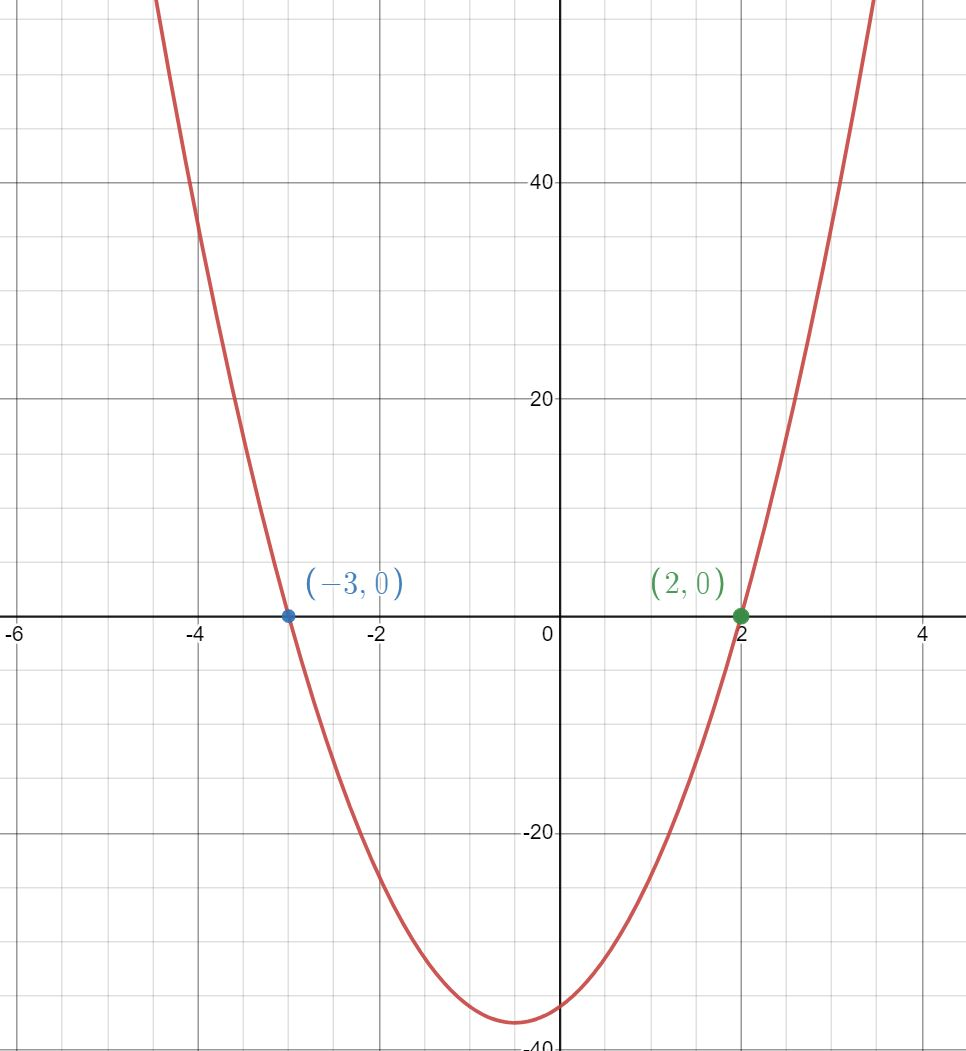
\includegraphics[height=5cm, width=9cm]{one.JPG}
      }

  \end{enumerate}

  \rule{15cm}{1pt}

  \textbf{4.4 L'HOSPITAL'S RLILE AND THE INVERSE-FUNCTION THEOREM}
  \begin{enumerate}
    \item (32) Assume the rules for differentiating the elementary functions, and use L'Hospital's Rule
    and find the following limits: 
    \begin{enumerate}
      \item $\lim\limits_{x \to 1} \dfrac{ln(x)}{x-1}$

        \textcolor{hwColor}{
          $
            \lim\limits_{x \to 1} \dfrac{ln(x)}{x-1}
            =\lim\limits_{x \to 1} \dfrac{\dfrac{1}{x}}{1-0}
            =\dfrac{\dfrac{1}{1}}{1-0}
            \\
            \\
            \\
            \therefore ~~~~ \lim\limits_{x \to 1} \dfrac{ln(x)}{x-1}=1 ~~~~ \checkmark
            \\
          $
        }

      \item $\lim\limits_{x \to 0} \dfrac{x}{e^x-1}$

        \textcolor{hwColor}{
          $
            \lim\limits_{x \to 0} \dfrac{x}{e^x-1}
            =\lim\limits_{x \to 0} \dfrac{1}{e^x-0}
            =\dfrac{1}{e^0-0}
            \\
            \\
            \\
            \therefore ~~~~ \lim\limits_{x \to 0} \dfrac{x}{e^x-1}=1 ~~~~ \checkmark
            \\
          $
        }

      \item $\lim\limits_{x \to 0} \dfrac{sin(x)}{x}$

        \textcolor{hwColor}{
          $
            \lim\limits_{x \to 0} \dfrac{sin(x)}{x}
            =\lim\limits_{x \to 0} \dfrac{cos(x)}{1}
            =\dfrac{cos(0)}{1}
            \\
            \\
            \\
            \therefore ~~~~ \lim\limits_{x \to 0} \dfrac{sin(x)}{x}=1 ~~~~ \checkmark
            \\
          $
        }

    \end{enumerate}

    \pagebreak

    \item (33) Use L'Hospitd's Rule to find the limit:
    $$
      \lim\limits_{x \to 0} \dfrac{x^2 sin(x)}{sin(x)-x cos(x)}
    $$

      \textcolor{hwColor}{
        $
          \lim\limits_{x \to 0} \dfrac{x^2 sin(x)}{sin(x)-x cos(x)}
          \\
          \\
          =\lim\limits_{x \to 0} \dfrac{2x sin(x)+x^2 cos(x)}{cos(x)-\left[cos(x)-xsin(x)\right]}
          \\
          \\
          =\lim\limits_{x \to 0}  
        $
      }

    \item (39) Suppose $f: R \longrightarrow R$ is such that $f(x+y)=f(x)f(y), f$ is differentiable at zero, and $f$ is
    not identically zero. Prove that $f$ is differentiable everywhere and that $f^'(x)=f(x)f^'(0)$.
    Assuming the properties of the exponential function, prove that $f(x)=e^{cx}$ where $c=f^'(0)$.

      \textcolor{hwColor}{
        Suppose $x=0$ and $y=0$.
        \\
        \\
        $
          f(x+y)=f(x) f(y) \Longrightarrow f(0)=f(0)^2
          \\
          \\
          \\
          \therefore ~~~~ \begin{cases}
            f(0)=0
            \\
            f(0)=1
          \end{cases}
          \\
          \\
          \dfrac{d}{dx} \left[f(0)\right]=\lim\limits_{x \to 0} \dfrac{f(t)-f(0)}{t}=\lim\limits_{x \to 0} \dfrac{f(t)-1}{t}
          \\
          \\
          \\
          \dfrac{df}{dx}=\lim\limits_{x \to 0} \dfrac{f(x_0+t)-f(x_0)}{t}=f(x_0) f^'(0) ~~~ \checkmark
        $
        \\
        \\
        Based on what we just showed $f(x)$ is differentiable everywhere.
        \\
        \\
        $
          \dfrac{df}{dx}=f(x) \dfrac{d}{dx} \left[f(0)\right]
          \\
          \\
          \dfrac{df}{f(x)}=xf^'(0)
          \\
          \\
          \\
          \therefore ~~~~ f(x)=e^{xf^'(0)} ~~~~ \checkmark
        $
      }

  \end{enumerate}
\end{document}
